\documentclass[12pt]{article}
\usepackage[russian]{babel}
\usepackage{geometry}

%библиотеки для задания 2
\usepackage{graphicx}
\usepackage{caption}

\usepackage{enumitem}

%нестандартные математические обозначения
\usepackage{amssymb}
\usepackage{amsmath}

%различные цветовые модели
\usepackage[usenames]{color}
\usepackage[dvipsnames,table]{xcolor}
\usepackage{colortbl}

\usepackage{listings}
\usepackage{listingsutf8}
\usepackage[T2A]{fontenc}
\newcommand{\listingsttfamily}{\usefont{T2A}{PTMono-TLF}{m}{n}}

\lstset{
	language=C,                % choose the language of the code
	numbers=left,                   % where to put the line-numbers
	stepnumber=1,                   % the step between two line-numbers.        
	numbersep=5pt,                  % how far the line-numbers are from the code
	backgroundcolor=\color{black},  % choose the background color. You must add \usepackage{color}
	commentstyle=\color{Gray},
	basicstyle=\listingsttfamily\color{Gray},
	keywordstyle=\color{BurntOrange},
	stringstyle=\color{YellowGreen},
	showspaces=false,               % show spaces adding particular underscores
	showstringspaces=false,         % underline spaces within strings
	showtabs=false,                 % show tabs within strings adding particular underscores
	tabsize=4,                      % sets default tabsize to 2 spaces
	captionpos=b,                   % sets the caption-position to bottom
	breaklines=true,                % sets automatic line breaking
	breakatwhitespace=true,         % sets if automatic breaks should only happen at whitespace
	title=\lstname, 
	inputencoding=utf8,                % show the filename of files included with \lstinputlisting;
	extendedchars=\true,
	keepspaces=true
}

%параметры документа
\geometry{top=2cm, bottom=2cm, left=1cm, right=1cm}
\textheight=24cm
\textwidth=18cm
\flushbottom 

\oddsidemargin=0pt 
\topmargin=-1.5cm 
\parskip=0pt
\parindent=24pt 

\tolerance=2000 

\begin{document}
	\begin{center}
		{\parskip=1cm
			МИНИСТЕРСТВО НАУКИ И ВЫСШЕГО ОБРАЗОВАНИЯ РОССИЙСКОЙ ФЕДЕРАЦИИ
			
			ФЕДЕРАЛЬНОЕ ГОСУДАРСТВЕННОЕ БЮДЖЕТНОЕ ОБРАЗОВАТЕЛЬНОЕ УЧРЕЖДЕНИЕ ВЫСШЕГО ОБРАЗОВАНИЯ
			
			{\bf«БЕЛГОРОДСКИЙ ГОСУДАРСТВЕННЫЙ ТЕХНОЛОГИЧЕСКИЙ УНИВЕРСИТЕТ им. В. Г. Шухова»\\(БГТУ им. В. Г. Шухова)}
			
			
			\begin{figure}[bh]
			\noindent\centering{
				
\includegraphics[width=100mm]{images/start_logo.png}
				\captionsetup{labelformat=empty}
			}
			\end{figure}
			Кафедра программного обеспечения вычислительной техники и автоматизированных систем
		}
		{\parskip=0.25cm
			{\Large 
				{\bf Лабораторная работа №5}
			
				по дисциплине: <<Алгоритмы и структуры данных>>
			
				по теме: {\bf <<Структуры данных <<линейные списки>> (С)>>}
			}
		}
	\end{center}
	\begin{flushright}
		{\parskip=3cm Выполнил/a: ст. группы ПВ-231}
		
		Чупахина София Александровна
		
		Проверил:
		
		Акиньшин Даниил Иванович
	\end{flushright}
	\begin{center}
		{\parskip=3cm Белгород, 2024}
	\end{center}
	\newpage
	
	{\bf Цель работы:} изучить СД типа <<линейный список>>, научиться их программно реализовывать и использовать.
	
	
	{\bf Задания:}
	
	\setlist[3]{noitemsep} % sets the itemsep and parsep for all level two lists to 0
	
	\begin{enumerate}
	
	\item Для СД типа <<линейный список>> определить:
	
		\begin{enumerate}
	
			\item Абстрактный уровень представления СД:
			
			\begin{enumerate}
	
				\item Характер организованности и изменчивости, 
	
				\item Набор допустимых операций.
			
			\end{enumerate}
	
	
			\item Физический уровень представления СД:
			
			\begin{enumerate}
	
				\item Схему хранения;
	
				\item Объем памяти, занимаемый экземпляром СД;
	
				\item Формат внутреннего представления СД и способ его  интерпретации;
				
				\item Характеристику допустимых значений;
				
				\item Тип доступа к элементам.
				
			\end{enumerate}
			
			\item Логический уровень представления СД. Способ описания СД и экземпляра СД на языке программирования.
	
		\end{enumerate}
	
	\item Реализовать СД типа «линейный список» в соответствии с вариантом индивидуального задания (см. табл.14) в виде модуля;
	
	\item Разработать программу для решения задачи в соответствии с вариантом индивидуального задания (см. табл.14) с использованием модуля, полученного в результате выполнения пункта 2 задания.
	
	\end{enumerate}
	
	\setcounter{secnumdepth}{-1} 
	\tableofcontents
	\newpage
	
	{\parskip=0.15cm
	
	\section{Задание 1:}
	\label{task_1}
	Опишем СД типа <<линейный список>>.
	
	\subsection{Абстрактный уровень:}
	\label{task_1_1}
	\subsubsection{Задание 1.1.1:}
	\label{task_1_1_1}
	
	СД типа <<линейный список>> является линейной СД (что, собственно, и отражено в её названии). Она, как и массив, отображает некую последовательность элементов: эти элементы находятся в линейном порядке, и для каждого из них, кроме первого и последнего, существует предыдущий и следующий. СД типа <<линейный список>> может быть реализована для любого типа элементов. Можно сказать, что на абстрактном уровне СД типа <<линейный список>> и СД типа массив схожи, различия появляются на физическом и логическом уровнях; обе СД хранят последовательности элементов, но выбраны разные способы их представления и сохранения упорядоченности с памяти компьютера. 
	
	Линейный список является динамической СД: в нем могут меняться как сами элементы, так и их количество. Причем, в отличие от массива, это количество не обязательно ограничено количеством элементов, под которые память была выделена при инициализации (это зависит от того, какая схема хранения была выбрана для реализации структуры; этот аспект подробнее рассмотрим в задании 1.2). К каждому элементу списка можно обратиться, зная его место в списке (индекс) и перезаписать его значение, однако процесс поиска элемента с данным индексом будет отличаться от такового в массиве (что, опять-таки, будет рассмотрено далее).
	
	\subsubsection{Задание 1.1.2:}
	\label{task_1_1_2}
	В отличие от СД, рассматриваемых в прошлых лабораторных работах, СД типа <<линейный список>> является не встроенной, а производной, то есть не реализована в языках программирования по умолчанию. Тем не менее, для линейного списка определен набор обязательных операций:
	\begin{enumerate}
	\item Инициализация.
	\item Включение элемента.
	\item Исключение элемента.
	\item Чтение текущего элемента.
	\item Переход в начало списка.
	\item Переход в конец списка.
	\item Переход к следующему элементу.
	\item Переход к i-му элементу.
	\item Определение длины списка.
	\item Уничтожение списка.
	\end{enumerate}
	
	\subsection{Физический уровень:}
	\label{task_1_2}
	\subsubsection{Задание 1.2.1:}
	\label{task_1_2_1}
	Здесь мы подходим к основному отличию СД типа массив и СД типа <<линейный список>>. В отличие от массива, который всегда имеет прямоугольную схему хранения, линейный список может быть реализован как при прямоугольной, так и при связной схеме хранения. С прямоугольной схемой мы уже знакомы: при ее использовании все элементы СД хранятся в памяти компьютера последовательно: последовательности битов, представляющие нулевой, первый, второй и так далее элемент, идут друг за другом по возрастанию адреса без разделителей. Линейный список, использующий эту схему, называется последовательным линейным списком (ПЛС). При связной же схеме хранения каждый элемент не просто хранит некоторое значение --- часть последовательности, а является элементом типа <<запись>> (такие элементы также называют узлами), куда кроме непосредственно значения записаны еще и адреса других элементов списка. Список, реализованный с помощью этой схемы, называется связным линейным списком (СЛС); связные линейные списки делятся на группы и далее, в зависимости от количества указателей, которые содержит тип <<запись>>. Если указатель один и для каждого элемента указывает на следующий/предыдущий элемент, то линейный список называется односвязным (ОЛС). Если указателей два, и один указывает на предыдущий, а второй --- на следующий, то линейный список называется двусвязным (ДЛС). Если же каждый элемент содержит множество указателей на элементы, являющиеся частью последовательности, объединенной каким-либо признаком, то линейный список называется многосвязным. Связные линейные списки, тем не менее, также могут быть реализованы с использованием статической памяти и массивов.
	\subsubsection{Задание 1.2.2:}
	\label{task_1_2_2}
	Количество памяти, занимаемой списком, зависит от того, какое количество памяти занимает его базовый тип в частности и тип <<запись>> (для СЛС) в целом и сколько элементов содержит список. Если базовый тип занимает $T$ байт, указатель (типа {\it unsigned long}) --- 8 байт, а список содержит $K$ элементов, то для ОЛС количество памяти, занимаемой экземпляром, будет равно $(T+8)*K$ байт, для ДЛС $(T+16)*K$ байт, для не использующих указатели ПЛС $T*K$ байт.
	
	\subsubsection{Задание 1.2.3:}
	\label{task_1_2_3}
	Если линейный список с длиной K является последовательным, то значение этой структуры хранится как K идущих подряд последовательностей битов, кодирующих значения элементов списка в соответствии с правилами для данного базового типа. Для связных же списков каждый узел хранится независимо друг от друга. Сами по себе узлы являются структурами, где одно поле отведено для хранения значения элемента (способ перевода в двоичный код зависит от базового типа), а одно, два или несколько полей --- указателями на следующий узел (указатели кодируются как положительные целые числа --- переводятся в двоичную систему счисления и дополняются нулями слева до размера в 8 байт). Двоичные коды значений отдельных полей структур также могут храниться в памяти компьютера не подряд (либо в порядке, отличном от заданного). Также связный линейный список может обладать фиктивными узлами, то есть узлами, где поле данных пусто, в его концах --- одним узлом для ОЛС и двумя узлами для ДЛС.

	\subsubsection{Задание 1.2.4:}
	\label{task_1_2_4}
	Диапазон допустимых значений линейного списка также связан с диапазоном допустимых значений его базового элемента. Однако всегда можно точно сказать, что количество возможных значений для линейного списка определенной длины K равно возведенному в степень K количеству возможных значений для его базового элемента. Соответственно, для СД типа <<линейный список>> количество возможных значений равно сумме количеств возможных значений списков с длинами от 0 до max, где max --- максимальная длина списка (однозначно определенная в случаях, когда линейный список реализован на массиве). Обозначая количество допустимых значений как CAR (кардинальное число), получим формулу $CAR(ЛС) = CAR(BaseType)^0 + CAR(BaseType)^1 +… + CAR(BaseType)^max$.
	
	\subsubsection{Задание 1.2.5:}
	\label{task_1_2_5}
	Для последовательных линейных списков, использующих для хранения элементов массивы, доступ к элементам является прямым --- при заданном индексе элемента, его адрес находится за фиксированное, не связанное с этим индексом число операций. Для связных линейных списков, использующих <<записи>> и систему указателей, связывающую соседние элементы, доступ к элементам является последовательным: необходимо идти от первого элемента к тому, с которым он связан, и так до тех пор, пока не будет достигнут требуемый.
	
	\subsection{Логический уровень:}
	\label{task_1_3}
	СД типа <<линейный список>> не является встроенной, и потому описать его на логическом уровне (представить на языке программирования) можно только для определенной реализации. Приведем здесь описание для той реализации, которая будет выполнена в задании 2 этой лабораторной работы --- то есть для односвязного линейного списка на массиве.
	
	\lstinputlisting{../АСД 5 си/example.c} 
	
	Увы, из-за отсутствия функций, облегчающих заполнение массива записями и вообще изменение полей списка (они будут реализованы в задании 2), она выглядит несколько громоздко. По сути здесь мы объявляем тип базового элемента, создаем структуру-<<запись>>, хранящую значение базового типа и индекс (в массиве) элемента, идущего следующим в текущем списке, а потом создаем структуру-<<список>>, хранящую указатель на первый и текущий элементы и количество элементов в списке на данный момент. В заданном массиве ListsContainer хранятся два списка с элементами \{1, 5, 6, -7\} и \{3, 2\}. Начало первого списка --- элемент под индексом 1, второго --- элемент под индексом 8. Идя по элементам с индексами в полях next, начиная от стартового элемента, рано или поздно мы придем к элементу под индексом 0 --- началу списка свободных элементов. Увидеть, что элементы списков действительно связаны, помогает функция PrintList (мы можем увидеть результаты вывода на скриншоте ниже).
	
	\begin{figure}[bh]
		\noindent\centering{
			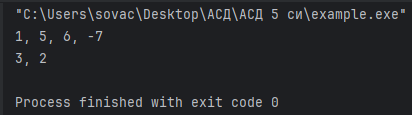
\includegraphics[width=110mm]{images/example.png}
			\captionsetup{labelformat=empty}
		}
	\end{figure}
	
	\newpage
	
	\begin{center}
	{\bf Индивидуальное задание; вариант 21}
	\end{center}
	{\bf Модуль 5:} Элементы ОЛС находятся в массиве {\it Memlist}, расположенном в статической памяти. Базовый тип зависит от задачи. «Свободные» элементы массива объединяются в список, на начало которого указывает поле-указатель первого элемента массива. Выделение памяти под информационную часть элемента  ОЛС и запись в нее значения происходит при выполнении процедуры {\it PutList}. При выполнении процедуры {\it GetList} память, занимаемая  элементом, освобождается.
	{\bf Реализация на языке C:}
	
	{\it \#if !defined(\_\_LIST5\_H)
	
	\#define   SizeList    100
	const short ListOk = 0;
	
	const short ListNotMem = 1;
	
	const short ListUnder = 2;
	
	const short ListEnd  = 3;
	
	typedef <определить>  BaseType;
	
	typedef   unsigned ptrel;
	
	typedef   struct element \{basetype data;
		ptrel next; \}; 
		
	typedef   struct List \{ptrel Start; 
		ptrel ptr;
		unsigned int N\}
		
	element MemList[SizeList];
	
	short   ListError;
	
	void InitList(List *L)
	
	void PutList(List *L, BaseType E)
	
	void GetList(List *L, BaseType *E)
	
	void ReadList(List *L,BaseType *E)
	
	int FullList(List *L)
	
	int EndList(List *L)
	
	usigned int Count(List *L)
	
	void BeginPtr(List *L)
	
	void EndPtr(List *L)
	
	void MovePtr(List *L)
	
	void MoveTo(List *L, unsigned int n)
	
	void DoneList(List *L)
	
	void CopyList(List *L1,List *L2)
	
	void InitMem()/*присваивает Flag каждoго элемента в 0*/
	
	int EmptyMem() /*возвращает 1, если в массиве нет свободных элементов*/
	
	unsigned  NewMem()//возвращает номер свободного элемента
	
	void DisposeMem(unsigned n) /*делает n-й элемент масcива cвободным*/
	
	\#endif}
	
	{\bf Задача 10:} Проверить,  удовлетворяют ли элементы списка (базовый тип {\it integer}) закону $x = f(х_0, h)$, где $х$ — элемент списка, $h$ — шаг, $x_0$ — начальный элемент списка.    
	Пример:  $x_0$ = 5, $h$ = 1. $x_1$ = 6, $x_2$ = 7, $x_3$ = 8... Элементы списка удовлетворяют закону $х = f(5, 1)$.
	
	\section{Задание 2:}
	\label{task_2}
	
	Разделим код выполнения этого задания на два файла: заголовочный и  реализации. В заголовочном файле зададим константы с кодами трех основных ошибок, которые могут возникнуть в ходе работы со списками: ListNotMem --- для выделения места под новый элемент нет места в списке свободных элементов в массиве MemList; ListUnder --- попытка получить доступ к элементу, в то время как пуст либо список, либо текущий указатель; ListEnd --- в ходе перебора элементов списка был достигнут его конец. Под хранение кода ошибки отводится переменная. После этого дадим название используемым типам данных: BaseType --- тип, элементы которого хранит список (в нашем случае это целые числа int); ptrel --- беззнаковое целое число, индекс элемента массива MemList, где хранится некоторый элемент; element --- запись, состоящая из значения элемента и индекса, по которому хранится следующий элемент; List --- структура, хранящая индексы начального и текущего элемента, а также их общее количество. Только после этого будут объявлены прототипы функций для работы со списками. 
	
	\lstinputlisting[linerange={1-62, 65-66}]{../АСД 5 си/List.h} 
	
	Реализация функций будет вынесена в отдельный файл со следующим содержанием.
	
	{\bf Примечание:} функция PutList подразумевает, что элемент вставляется после элемента, на который указывает рабочий указатель, поэтому, чтобы вставить элемент в самое начало списка, рабочий указатель должен быть равен нулю, при условии, что нулю не равен стартовый указатель (если же стартовый указатель равен 0, это запускает отдельный алгоритм вставки в пустой список).
	
	\lstinputlisting[linerange={1-173, 189-190}]{../АСД 5 си/List.c} 

	Для нормальных (не вызывающих ошибки и аварийного завершения) сценариев большинства функций (за исключением тех, что работают не со списками, а непосредственно с массивом MemList, на основе которого они хранятся, а также уничтожающей список функции DoneList), можно составить автоматизированные тесты и вынести их в отдельный файл тестирования. Будем тестировать функции по порядку; после того, как они протестированы, их можно использовать в тестах дальнейших функций.
	
	\lstinputlisting[linerange={1-446, 477-489, 492-498}]{../АСД 5 си/List_test.c} 
	
	Запустив программу, можем самостоятельно убедиться, что все тесты прошли успешно:
	
	\begin{figure}[bh]
		\noindent\centering{
			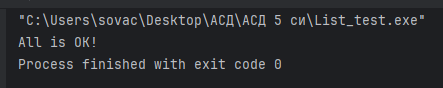
\includegraphics[width=150mm]{images/general_output.png}
			\captionsetup{labelformat=empty}
		}
	\end{figure}
	
	
	\section{Задание 3:}
	\label{task_3}
	
	Теперь, когда все функции, обязательные для СД типа <<линейный список>>, реализованы, можем решить задачу, в ходе которой нам предстоит работать с линейными списками. Прототип функции, решающей задачу добавим в заголовочный файл, затем вставим основной код в файл реализации, а в файле с автоматизированными тестами рассмотрим несколько сценариев: список содержит один элемент (будем считать, что тогда он удовлетворяет условию); список содержит несколько элементов, и шаг между ними одинаков и соответствует заданному; список содержит несколько элементов, но на одном из них шаг отклоняется от заданного, и часть последовательности после него перестает соответствовать условию.
	
	{\bf Примечание:} случай, когда последовательность пуста, будем считать ошибкой: программа аварийно завершает выполнение с кодом ListUnder.
	
	\lstinputlisting[linerange={174-188}]{../АСД 5 си/List.c} 
	
	\lstinputlisting[linerange={447-477, 490-498}]{../АСД 5 си/List_test.c} 
	
	Запустив программу, можем убедиться, что и этот тест полностью пройден:
	
	\begin{figure}[bh]
		\noindent\centering{
			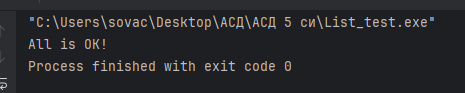
\includegraphics[width=150mm]{images/task_output.png}
			\captionsetup{labelformat=empty}
		}
	\end{figure}
	
	
	\section{Вывод:}
	
	В ходе лабораторной работы дали характеристику СД типа <<линейный список>> и ее подвидам (ПЛС, ОЛС, ДЛС), форматам их представления, реализовали один из них (односвязный линейный список на основе массива в статической памяти), написали ряд базовых функций для работы с односвязными линейными списками в этом формате.
	
}
\end{document}